{\color{gray}\hrule}
\begin{center}
\section{Methodology}
\textbf{Systematic Procedure to Identify Papers}
\bigskip
\end{center}
{\color{gray}\hrule}
\begin{multicols}{2}
The research process started with the defintion of the topic together with our supervisor Professor Pierson, together we decided to settle on creating a state fo the art review on the topic of Container and Cloud Computing, with a particular emphasis on energy consumption optimization. 
To begin with we defined a "Search Pipeline"


\begin{figure}[H]
    \centering
    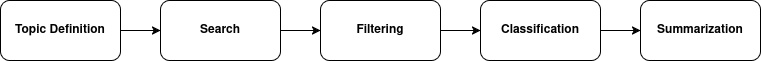
\includegraphics[width=\columnwidth]{flowchartTIR.png}
    \caption{Search Pipeline Flowchart}
    \label{fig:search_pipeline}
\end{figure}

This procedures allowed us to organize the work and have a standardized method of acceptance for navigating the papers. 
We also defined a search string with which we would start the search: ((energy OR resource) AND container).
We decided to expand the search also to resource since we noticed that many times better resource utilization leads to better dynamic power handling, hence lowering the amount of energy required to carry out a task.
Before starting with the research we also defined some acceptance criteria that would define whether a paper was going to be included in our survey or not. We defined the criteria as follows:



\begin{table}[H]
\centering
\begin{tabular}{c}
\hline
Direct Exclusion of Paper If \\ \hline
Work is not in English \\ 
Work is not a scientific paper \\ 
Work has less than 10 citations \\ 
Work is not about containers/cloud \\ \hline
\end{tabular}
    \caption{Exclusion Rules}
    \label{tab:Exclusion Rules}
\end{table}

Hence we proceeded with our search and we identified a total of 34 papers. That are divided as follows through the various publishers

\begin{figure}[H]
    \centering
    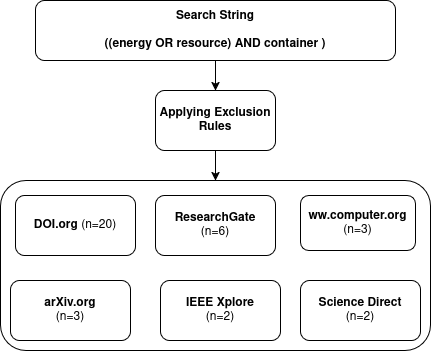
\includegraphics[width=\columnwidth]{sections/exportedPapers.png}
    \caption{Exported Papers}
    \label{fig:search_pipeline}
\end{figure}

To have an insight on the publication dates for the filtered papers, we can clearly visualize how the period between 2017 and 2019 was the most important for research in this field.

\begin{figure}[H]
    \centering
    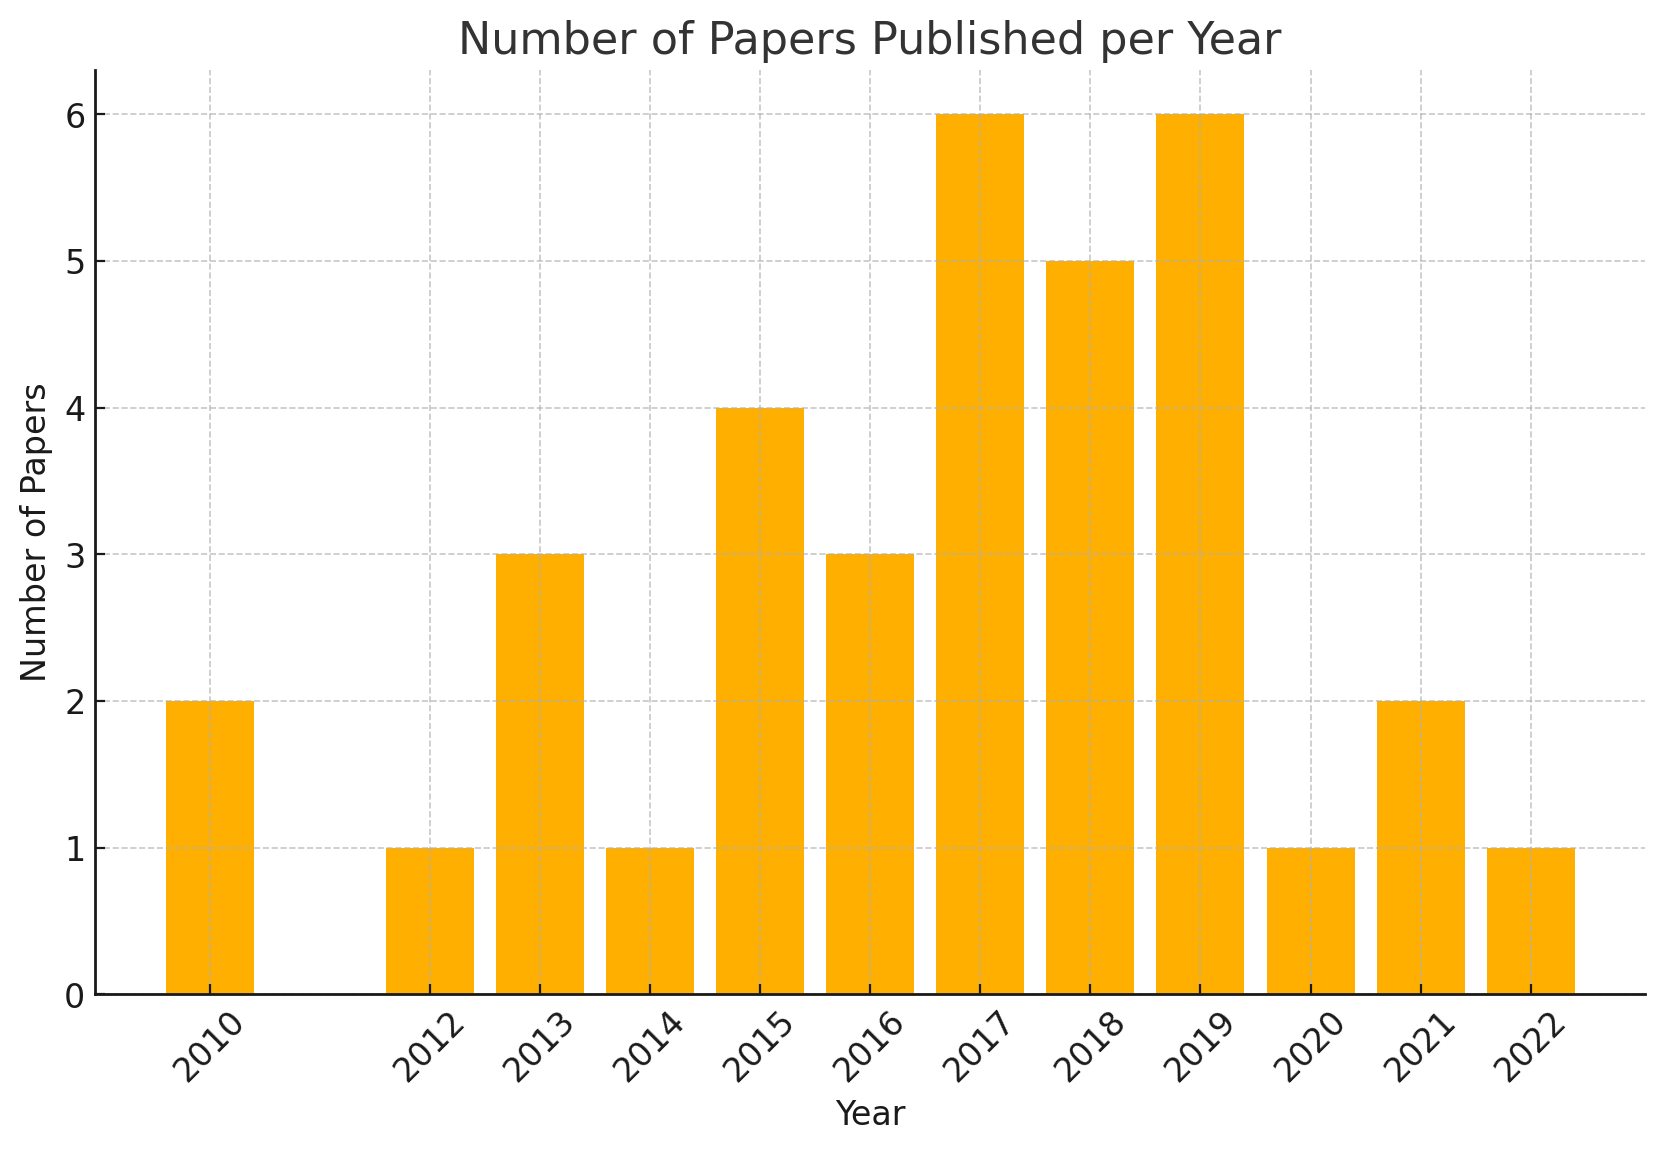
\includegraphics[width=\columnwidth]{papers_per_year.png}
    \caption{Papers per year}
    \label{fig:search_pipeline}
\end{figure}

At this point we could move to the classification step of our workflow. We decided to define the following  metrics

\begin{table}[H]
\centering
\begin{tabular}{c c}
\hline
Direct Exclusion of Paper If \\ \hline
Work is not in English \\ 
Work is not a scientific paper \\ 
Work has less than 10 citations \\ 
Work is not about containers/cloud \\ \hline
\end{tabular}
    \caption{Exclusion Rules}
    \label{tab:Exclusion Rules}
\end{table}

\end{multicols}